\documentclass[9pt,onecolumn,twoside,]{pinp}

%% Some pieces required from the pandoc template
\providecommand{\tightlist}{%
  \setlength{\itemsep}{0pt}\setlength{\parskip}{0pt}}

% Use the lineno option to display guide line numbers if required.
% Note that the use of elements such as single-column equations
% may affect the guide line number alignment.

\usepackage[T1]{fontenc}
\usepackage[utf8]{inputenc}

% pinp change: the geometry package layout settings need to be set here, not in pinp.cls
\geometry{layoutsize={0.95588\paperwidth,0.98864\paperheight},%
  layouthoffset=0.02206\paperwidth, layoutvoffset=0.00568\paperheight}

\definecolor{pinpblue}{HTML}{185FAF}  % imagecolorpicker on blue for new R logo
\definecolor{pnasbluetext}{RGB}{101,0,0} %



\title{Parcial 3}

\author[]{}


\setcounter{secnumdepth}{0}

% Please give the surname of the lead author for the running footer
\leadauthor{}

% Keywords are not mandatory, but authors are strongly encouraged to provide them. If provided, please include two to five keywords, separated by the pipe symbol, e.g:
 

\begin{abstract}

\end{abstract}

\dates{This version was compiled on \today} 

% initially we use doi so keep for backwards compatibility
% new name is doi_footer


\begin{document}

% Optional adjustment to line up main text (after abstract) of first page with line numbers, when using both lineno and twocolumn options.
% You should only change this length when you've finalised the article contents.
\verticaladjustment{-2pt}

\maketitle
\thispagestyle{firststyle}
\ifthenelse{\boolean{shortarticle}}{\ifthenelse{\boolean{singlecolumn}}{\abscontentformatted}{\abscontent}}{}

% If your first paragraph (i.e. with the \dropcap) contains a list environment (quote, quotation, theorem, definition, enumerate, itemize...), the line after the list may have some extra indentation. If this is the case, add \parshape=0 to the end of the list environment.


\hypertarget{calculo-del-volumen-usando-la-ecuaciuxf3n-de-smalian}{%
\section{1) Calculo del volumen usando la ecuación de
Smalian}\label{calculo-del-volumen-usando-la-ecuaciuxf3n-de-smalian}}

\[V_t= [\sum_{i=1}^{n}{(d_i^2+d_{i+1}^2)* (L_{i+1}-L_{i}})] * \frac{\pi}{8}\]

\hypertarget{seleccuxf3n-de-muestras-aleatorias-para-construcciuxf3n-de-modelos}{%
\section{2) Seleccón de muestras aleatorias para construcción de
modelos}\label{seleccuxf3n-de-muestras-aleatorias-para-construcciuxf3n-de-modelos}}

\hypertarget{modelos-de-volumen}{%
\subsection{3) Modelos de volumen}\label{modelos-de-volumen}}

El mejor modelo escogido es el 4, pues su \(RSE\) es el menor de todos
lo modelos.

los lineales no cumplen supuestos, mirar grafica de residuales para
mirar tendencia log.

\begin{table}

\caption{\label{tab:unnamed-chunk-9}Comparación de modelos}
\centering
\begin{tabular}[t]{l|r|l|r|r|r|r}
\hline
Modelo & Fc & valor.p & Shapiro & R.squared & AIC & RSE\\
\hline
V= 7.61e-01+(-1.30e-02*D+
               (8.69e-04*D\textasciicircum{}2)+(-1.09e-01*H)+
               (4.19e-03*H\textasciicircum{}2) & 395.9044 & *** & 0.0000 & 0.9577 & -53.01262 & 0.1623729\\
\hline
V= 2.44e-02+3.72e-05*(D\textasciicircum{}2*H) & 2336.9484 & *** & 0.0000 & 0.9697 & -84.11330 & 0.1345016\\
\hline
V= 6.40e-04*D\textasciicircum{}6.15*H\textasciicircum{}3.28 & 2444.2628 & *** & 0.8866 & 0.9855 & -74.91925 & 14.3482000\\
\hline
V= 5.88e-05*(D\textasciicircum{}2*H)\textasciicircum{}2.61 & 4304.9706 & *** & 0.3458 & 0.9833 & -66.51527 & 0.1320000\\
\hline
\end{tabular}
\end{table}

\begin{center}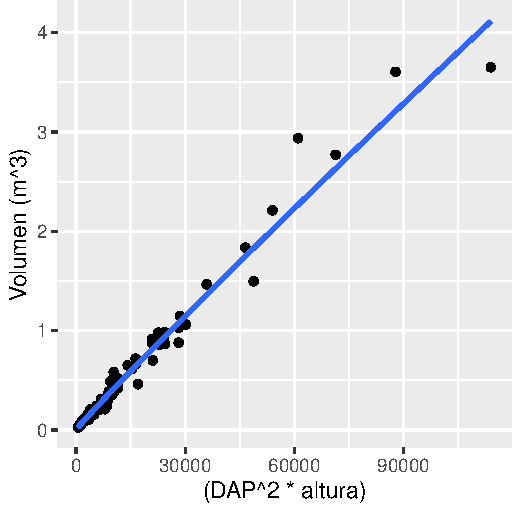
\includegraphics{David_Londono_Lopera_Cristian_Ganan_parcial3_files/figure-latex/unnamed-chunk-10-1} \end{center}

\begin{table}

\caption{\label{tab:unnamed-chunk-11}Validación de modelos volumen}
\centering
\begin{tabular}[t]{r|r|r|r}
\hline
Media3 & sd3 & Media4 & sd4\\
\hline
-1520.335 & 185.554 & -3.03686 & 14.20831\\
\hline
\end{tabular}
\end{table}

\hypertarget{calculo-de-biomasa}{%
\section{4) Calculo de biomasa}\label{calculo-de-biomasa}}

\hypertarget{modelos-de-biomasa-uxe1erea}{%
\section{5) Modelos de biomasa
áerea}\label{modelos-de-biomasa-uxe1erea}}

se presentan los modelos

\begin{center}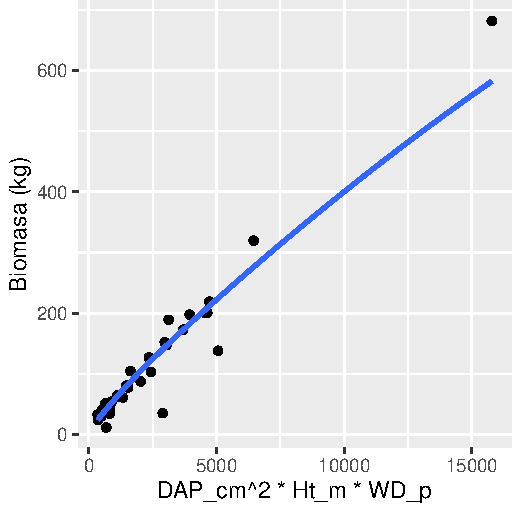
\includegraphics{David_Londono_Lopera_Cristian_Ganan_parcial3_files/figure-latex/unnamed-chunk-23-1} \end{center}

\begin{table}

\caption{\label{tab:unnamed-chunk-24}Modelos de Biomasa}
\centering
\begin{tabular}[t]{l|r|l|r|r|r|r}
\hline
Modelo & Fc & valor.p & Shapiro & R.squared & AIC & RSE\\
\hline
BA= -207.20+18.34*D+(-0.3342*H) & 39.6762 & *** & 0.0201 & 0.7829 & 286.14189 & 67.20959\\
\hline
BA= 3.75+0.025*(D\textasciicircum{}2*H) & 308.0868 & *** & 0.0032 & 0.9305 & 255.65875 & 37.18581\\
\hline
BA= 0.12*D\textasciicircum{}15.31*H\textasciicircum{}0.62 & 55.6392 & *** & 0.0073 & 0.8349 & 28.44571 & 52.93970\\
\hline
BA= 0.16*D\textasciicircum{}11.33*H\textasciicircum{}0.93*WD\textasciicircum{}2.16 & 51.5368 & *** & 0.0000 & 0.8513 & 29.23174 & 41.89810\\
\hline
BA= 0.23*(D\textasciicircum{}2*WD)\textasciicircum{}3.23 & 161.7459 & *** & 0.0000 & 0.8480 & 25.92556 & 40.08310\\
\hline
BA= 0.10*(D\textasciicircum{}2*H)\textasciicircum{}2.32 & 111.2088 & *** & 0.0000 & 0.7932 & 35.46763 & 42.46070\\
\hline
BA= 0.18*(D\textasciicircum{}2*H*WD)\textasciicircum{}2.31 & 91.9029 & *** & 0.0000 & 0.7998 & 31.26584 & 38.53990\\
\hline
\end{tabular}
\end{table}

\begin{ShadedResult}
\begin{verbatim}
#      Media_g     sd_e
#  1 -11.85311 26.66373
\end{verbatim}
\end{ShadedResult}
\begin{table}

\caption{\label{tab:unnamed-chunk-25}Validación de modelo Biomasa}
\centering
\begin{tabular}[t]{r|r}
\hline
Media\_g & sd\_e\\
\hline
-11.85311 & 26.66373\\
\hline
\end{tabular}
\end{table}

\hypertarget{estimacuxf3n-de-volumen-y-biomasa-en-cinco-localidades}{%
\subsection{6) Estimacón de volumen y biomasa en cinco
localidades}\label{estimacuxf3n-de-volumen-y-biomasa-en-cinco-localidades}}

\begin{table}

\caption{\label{tab:unnamed-chunk-29}Volumen del inventario}
\centering
\begin{tabular}[t]{r|r}
\hline
Media & Desviacion\\
\hline
77.58832 & 103.0507\\
\hline
\end{tabular}
\end{table}

\begin{table}

\caption{\label{tab:unnamed-chunk-30}Contenido de Carbono del iventario}
\centering
\begin{tabular}[t]{r|r}
\hline
media contenido de C & Sd contenido de C\\
\hline
2.175178 & 2.451563\\
\hline
\end{tabular}
\end{table}

\hypertarget{comparaciuxf3n-entre-localidades}{%
\section{7) Comparación entre
localidades}\label{comparaciuxf3n-entre-localidades}}

\begin{figure}

{\centering 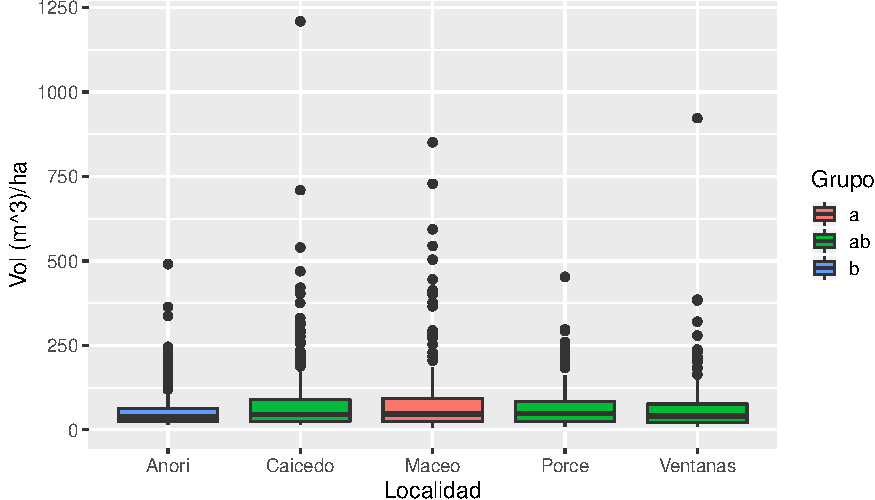
\includegraphics{David_Londono_Lopera_Cristian_Ganan_parcial3_files/figure-latex/unnamed-chunk-31-1} 

}

\caption{Comparación de volumen por Localidad}\label{fig:unnamed-chunk-31}
\end{figure}

\begin{figure}

{\centering 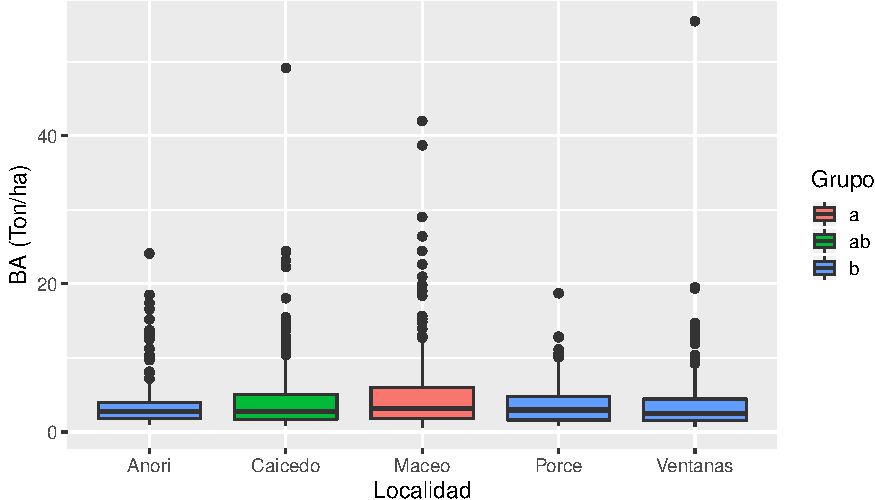
\includegraphics{David_Londono_Lopera_Cristian_Ganan_parcial3_files/figure-latex/unnamed-chunk-32-1} 

}

\caption{Comparación de Biomasa por Localidad}\label{fig:unnamed-chunk-32}
\end{figure}

\(BA \ = \ b_0 + b_1*D+b_2*H\) \(BA \ = \ b_0+b_1(D^2*H)\)
\(BA \ = \ b_0*D^{b_1}*H^{b_2}\)
\(BA \ = \ b_0*D^{b_1}*H^{b_2}*WD^{b_3}\)
\(BA \ = \ b_0*(D^2*WD)^{b_1}\) \(BA \ = \ b_0*(D^2*H)^{b_1}\)
\(BA \ = \ b_0*(D^2*H*WD)^{b_1}\)

%\showmatmethods

\pnasbreak 




\end{document}

